%-------------------------
% Resume in Latex
% Author : Shubhi Rani
% License : MIT
%------------------------

\documentclass[letterpaper,10.8pt]{article}

\usepackage{latexsym}
\usepackage[empty]{fullpage}
\usepackage{titlesec}
\usepackage{marvosym}
\usepackage[usenames,dvipsnames]{color}
\usepackage{verbatim}
\usepackage{enumitem}
\usepackage[pdftex]{hyperref}
\usepackage{fancyhdr}
\usepackage{pdfpages}


\pagestyle{fancy}
\fancyhf{} % clear all header and footer fields
\fancyfoot{}
\renewcommand{\headrulewidth}{0pt}
\renewcommand{\footrulewidth}{0pt}

% Adjust margins
\addtolength{\oddsidemargin}{-0.375in}
\addtolength{\evensidemargin}{-0.375in}
\addtolength{\textwidth}{1in}
\addtolength{\topmargin}{-.5in}
\addtolength{\textheight}{1in}

\urlstyle{rm}

\raggedbottom
\raggedright
\setlength{\tabcolsep}{0in}

% Sections formatting
\titleformat{\section}{
  \vspace{-3pt}\scshape\raggedright\large
}{}{0em}{}[\color{black}\titlerule \vspace{-5pt}]

%-------------------------
% Custom commands
\newcommand{\resumeItem}[2]{
  \item\small{
    \textbf{#1}{: #2 \vspace{-2pt}}
  }
}

\newcommand{\resumeItemWithoutTitle}[1]{
  \item\small{
    {\vspace{-2pt}}
  }
}

\newcommand{\resumeSubheading}[4]{
  \vspace{-1pt}\item
    \begin{tabular*}{0.97\textwidth}{l@{\extracolsep{\fill}}r}
      \textbf{#1} & #2 \\
      \textit{\small#3} & \textit{\small #4} \\
    \end{tabular*}\vspace{-5pt}
}


\newcommand{\resumeSubItem}[2]{\resumeItem{#1}{#2}\vspace{-4pt}}

\renewcommand{\labelitemii}{$\circ$}

\newcommand{\resumeSubHeadingListStart}{\begin{itemize}[leftmargin=*]}
\newcommand{\resumeSubHeadingListEnd}{\end{itemize}}
\newcommand{\resumeItemListStart}{\begin{itemize}}
\newcommand{\resumeItemListEnd}{\end{itemize}\vspace{-5pt}}

%-------------------------------------------
%%%%%%  CV STARTS HERE  %%%%%%%%%%%%%%%%%%%%%%%%%%%%


\begin{document}

%----------HEADING-----------------
\begin{tabular*}{\textwidth}{l@{\extracolsep{\fill}}r}
  \textbf{{\LARGE Sami Alexander Taieb, 1th August 2001}} & Email : \href{mailto:info@taieb.de}{info@taieb.de}\\
  %\href{https://www.linkedin.com/in/shubhir/}{Linkedin: https://www.linkedin.com/in/shubhir/} & Mobile : +1-631-645-8315 \\
  \href{https://github.com/samitxb}{Github: https://github.com/samitxb} \\
\end{tabular*}

%------------About Me----------------
%\section{About Me}
%\resumeSubHeadingListStart
%    \resumeItem {Date and place of birth}{01. August 2001, Passau D-94034}
%    \resumeItem {Nationality}{German}
%    \resumeItem{Phone}{0179 4204694}
%\resumeSubHeadingListEnd


%-----------EDUCATION-----------------
\section{Education}
  \resumeSubHeadingListStart
    \resumeSubheading
      {Deggendorf University of Technology}{Deggendorf, D-94469}
      {Applied Computer Science, M.Sc.}{Since March 2023}
    \resumeSubheading
      {Deggendorf University of Technology}{Deggendorf, D-94469}
      {Applied Computer Science (Embedded Systems), B.Eng.}{October 2019 - May 2024}
      
%	   {\scriptsize \textit{Courses: Operating Systems, Analysis Of Algorithms, Artificial Intelligence, Machine Learning, Probability and Statistics and Network Security.}}
\resumeSubHeadingListEnd
	    
%
%--------PROGRAMMING SKILLS------------
\section{Skills Summary}
	\resumeSubHeadingListStart
	\resumeSubItem{Programming Skills (still in practice)}{C, C++, VHDL, SystemVerilog}
    \resumeSubItem{Programming Skills (some expirience)}{Java, Python, Matlab, C\#, R, TypeScript}
	%\resumeSubItem{Tools}{VirtualBox, GIT, Matlab, Postgres, }
\resumeSubHeadingListEnd



%-----------EXPERIENCE-----------------
\section{Experience}
  \resumeSubHeadingListStart
    \resumeSubheading
		{IC-Design Reinhard Gottinger GmbH}{Passau, D-94034}
		{Master Thesis - Supervisor: Dominik Seidl}{Since October 2024}

    \resumeSubheading
		{IC-Design Reinhard Gottinger GmbH}{Passau, D-94034}
		{Working Student - Supervisor: Reinhard Gottinger}{March 2024 - September 2024}
  
    \resumeSubheading
		{IC-Design Reinhard Gottinger GmbH}{Passau, D-94034}
		{Bachelor Thesis - Supervisor: Dominik Seidl}{October 2023 - January 2024}
		\resumeItemListStart
    \resumeItem{Design, implementation and operation of a PCIe interface for data transfer between a PolarFire FPGA and the NVIDIA Jetson}{}
    \begin{description}[font=$\bullet$]
    \item {Designing the hardware for an PolarFire FPGA on an Arrow Everest Evaluation Board}
    \item {PCIe IP-Core configuration and integration}
    \item {Implementation of a DMA-Transfer}
    \item {Implementation of a driver and an application for the NVIDIA Jetson}
    \end{description}
    \resumeItemListEnd
  
    \resumeSubheading
		{IC-Design Reinhard Gottinger GmbH}{Passau, D-94034}
		{Working Student - Supervisor: Dominik Seidl}{March 2022 - October 2023}
      
    \resumeSubheading
		{IC-Design Reinhard Gottinger GmbH}{Passau, D-94034}
		{Internship - Supervisor: Reinhard Gottinger}{October 2021 -  February 2022}
		\resumeItemListStart
    \resumeItem{Measuring the antenna characteristics of RFID transponders for the high and low frequency range}{}
    \begin{description}[font=$\bullet$]
    \item {Recording of measurements of low and high frequency RFID transponder coils with the Dira-Test measuring device of IC-Design Reinhard Gottinger GmbH for contactless measurement of RFID systems}
    \item {Selecting suitable parameters for the components located in the circuit of the measuring device}
    \item {Creation of a prototype antenna with self-wound coils to transmit better usable signal}
    \item {Qualitative comparison of the prototypes with the previous antennas}
    \item {Comparison of the evaluated measured values of the Dira-Test meter with the results of the Network Analyzer from Rohde und Schwarz and the DG8SAQ from SDR-Kits}
    \item {Investigation of the influence of different energy inputs on the resonant frequency of RFID transponder coils with the Network Analyzer from Rohde und Schwarz}
    \item {Investigation of the deviation from the quality as a function of the capacitance, inductance and resistance}
    \end{description}
    \resumeItemListEnd
\resumeSubHeadingListEnd

%-----------Sonstige Nachweise-----------------
\section{additional qualification}
\resumeSubHeadingListStart
\resumeSubItem{training of trainers (AdA - HWK)}{according to german quality standards (AEVO)}
\resumeSubItem{practical training (HWK)}{as part of the technical secondary school in the technical branch}
    \begin{description}[font=$\bullet$]
    \item{Measuring electrical quantities}
    \item{Generation and management of electrical energy}
    \item{Conversion of electrical energy into other forms of energy}
    \item{Digital technology}
    \item{SPS technology}
    \end{description}
\resumeSubHeadingListEnd


%-----------PROJECTS-----------------
\section{Academic Projects}
\resumeSubHeadingListStart
\resumeSubItem{MatLab Simulation}{Path of a sphere on a functional surface}
\resumeSubItem{PXE Boot Server}{Setting Up a PXE-Boot Server on a Virtual Machine}
\resumeSubItem{Self-Balancing Robot}{Self-Balancing Robot based on Lego NXT alike the inverted pendelum}
\resumeSubItem{Driver Programming}{Implementation of a  driver for a seven-segment display on Raspian OS}
\resumeSubItem{Financial Manager}{Implementation of a Financial Manager in Java combined with Scene Builder GUI and posgresql database}
\resumeSubItem{NVM-Manager}{Implementation of a Manager for non-volatile memory in C}
\resumeSubHeadingListEnd


\includepdf[pages=-]{AdA.pdf}
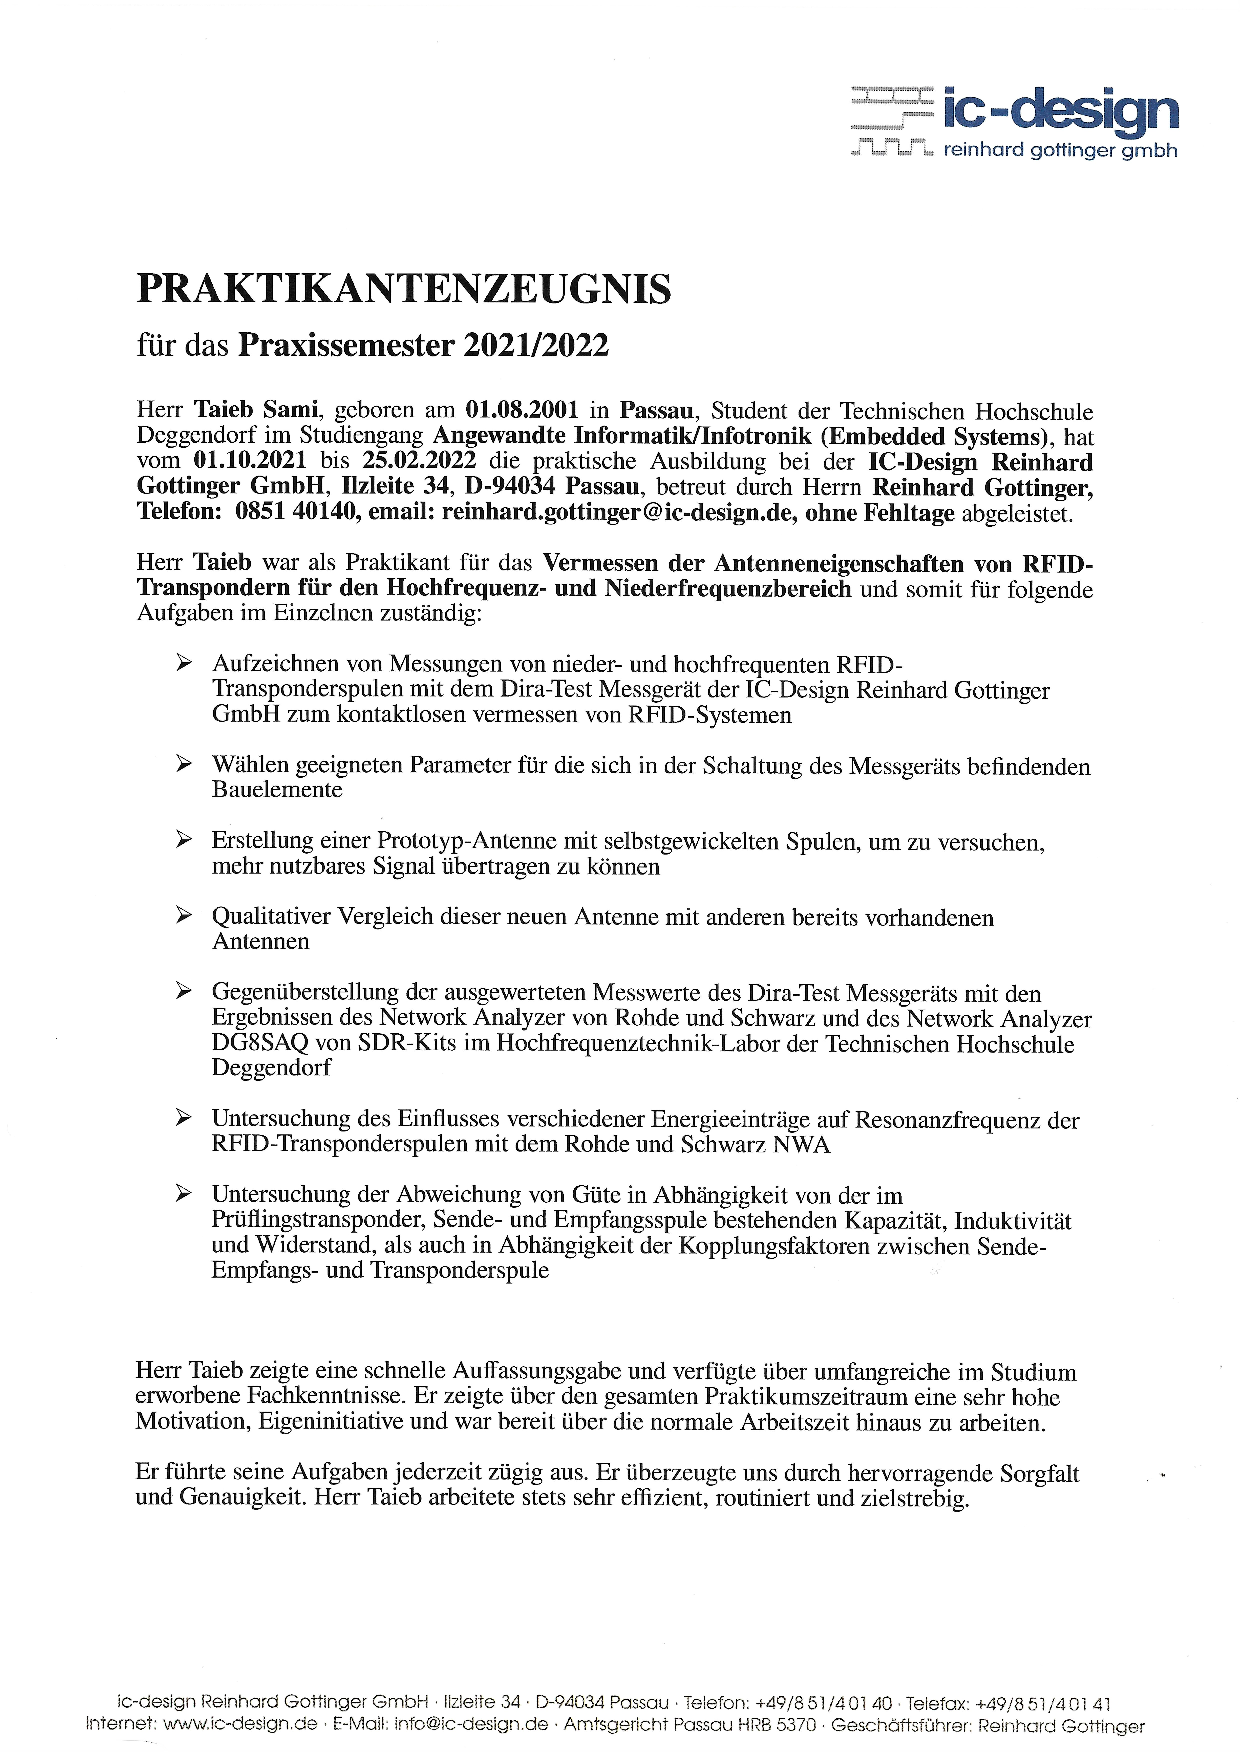
\includepdf[pages=-]{Praktikantenzeugnis Teil 1.pdf}

\includepdf[pages=-]{Praktikantenzeugnis Teil 2.pdf}
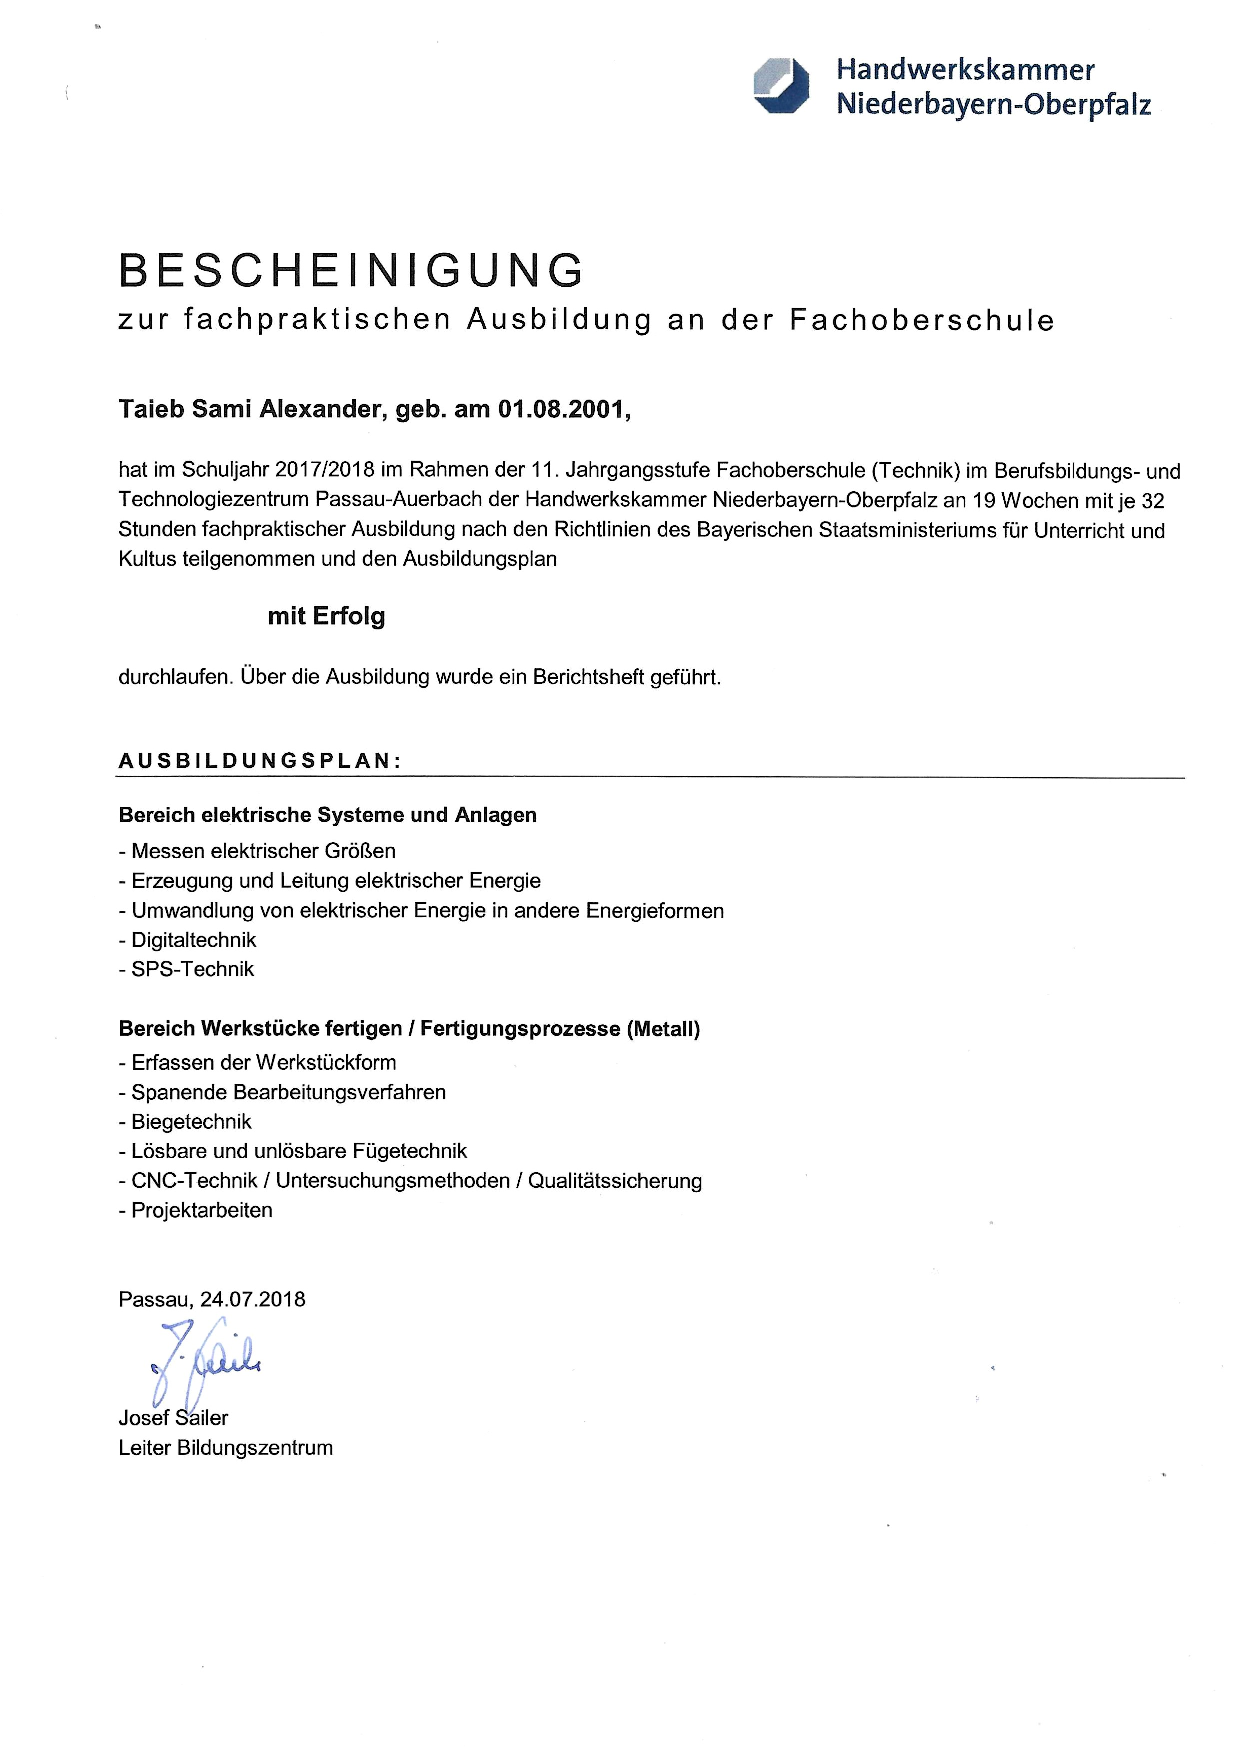
\includepdf[pages=-]{Handwerkskammer.pdf}

\end{document}